% Native TikZ figure. Required packages: tikz; graphicx for resizing.
% Horizontal positions and vertical levels are schematic, not to scale.
% Edit these coordinates to adjust the shape; displayed ratios are labels.
\begingroup
\definecolor{qsBlue}{HTML}{1769AA}
\definecolor{qsOrange}{HTML}{BE661D}
\definecolor{qsInk}{HTML}{263340}
\definecolor{qsGray}{HTML}{78828C}
\definecolor{qsGuide}{HTML}{B7C1CA}
\definecolor{qsGrid}{HTML}{E9EDF0}
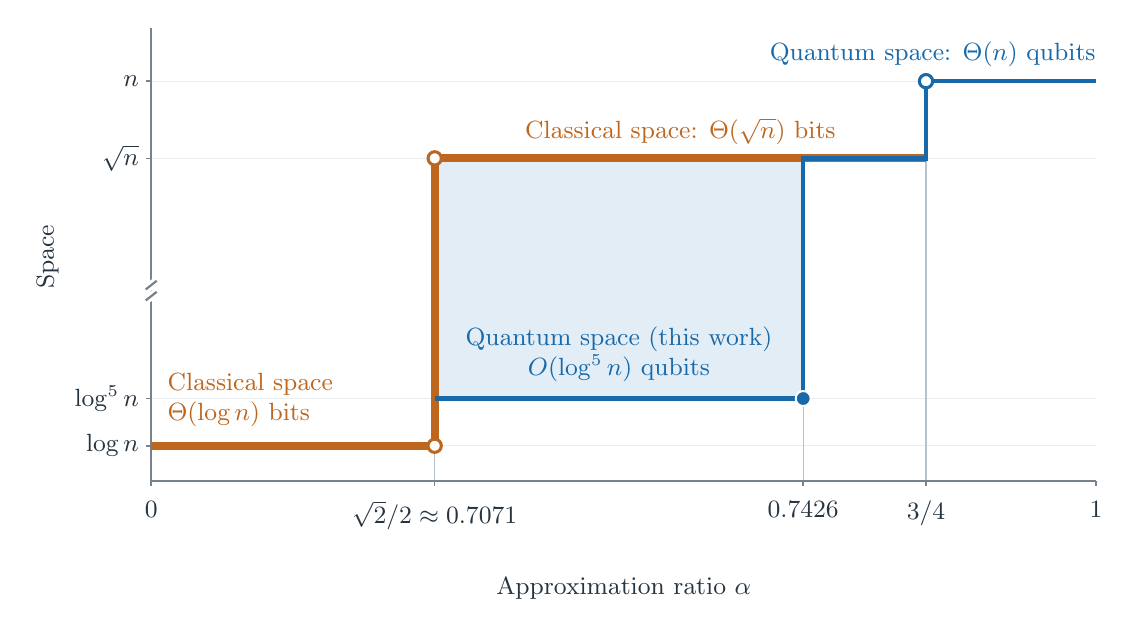
\begin{tikzpicture}[
  x=1cm, y=1cm, font=\small, text=qsInk,
  qs axis/.style={draw=qsGray,line width=.55pt},
  qs grid/.style={draw=qsGrid,line width=.4pt},
  qs guide/.style={draw=qsGuide,line width=.4pt},
  qs classical/.style={draw=qsOrange,line width=2.8pt,line cap=butt,line join=miter},
  qs quantum/.style={draw=qsBlue,line width=1.6pt,line cap=butt,line join=miter}
]
% Schematic threshold positions on the horizontal axis.
\def\xC{3.60}  % sqrt(2)/2
\def\xQ{8.28}  % 0.7426
\def\xT{9.84}  % 3/4
\def\xR{12.00} % 1
% Schematic asymptotic space levels.
\def\yLog{0.45}
\def\yPolylog{1.05}
\def\yRoot{4.10}
\def\yLinear{5.08}

% Advantage region; no descriptive text other than the quantum-space label.
\fill[qsBlue!12] (\xC,\yPolylog) rectangle (\xQ,\yRoot);
\foreach \yy in {\yLog,\yPolylog,\yRoot,\yLinear}
  \draw[qs grid] (0,\yy) -- (\xR,\yy);
\draw[qs guide] (\xC,0) -- (\xC,\yRoot);
\draw[qs guide] (\xQ,0) -- (\xQ,\yRoot);
\draw[qs guide] (\xT,0) -- (\xT,\yLinear);

% Axes and the vertical scale break.
\draw[qs axis] (0,5.75) -- (0,0) -- (\xR,0);
\foreach \yy in {2.35,2.49}
  \draw[white,line width=3pt] (-.07,\yy-.055) -- (.07,\yy+.055);
\foreach \yy in {2.35,2.49}
  \draw[qs axis,line width=.8pt] (-.07,\yy-.055) -- (.07,\yy+.055);

% Two continuous staircase paths. On the common segment the thinner blue
% stroke overlays orange, so both curves remain visible.
\draw[qs classical] (0,\yLog) -- (\xC,\yLog)
  -- (\xC,\yRoot) -- (\xT,\yRoot);
% The quantum step at xQ switches to the known classical upper bound.
% It is not a claim of a quantum lower bound at 0.7426.
\draw[qs quantum] (\xC,\yPolylog) -- (\xQ,\yPolylog)
  -- (\xQ,\yRoot) -- (\xT,\yRoot)
  -- (\xT,\yLinear) -- (\xR,\yLinear);

% Endpoints distinguish strict thresholds and the attained quantum ratio.
\filldraw[fill=white,draw=qsOrange,line width=1.1pt]
  (\xC,\yLog) circle[radius=2.4pt];
\filldraw[fill=white,draw=qsOrange,line width=1.1pt]
  (\xC,\yRoot) circle[radius=2.4pt];
\filldraw[fill=white,draw=qsBlue,line width=1.1pt]
  (\xT,\yLinear) circle[radius=2.4pt];
\filldraw[fill=qsBlue,draw=white,line width=.7pt]
  (\xQ,\yPolylog) circle[radius=2.7pt];

% Curve labels.
\node[anchor=south west,align=left,text=qsOrange,inner sep=0pt]
  at (.20,.68) {Classical space\\$\Theta(\log n)$ bits};
\node[anchor=south,align=center,text=qsBlue,inner sep=0pt]
  at (5.94,1.25) {Quantum space (this work)\\$O(\log^5 n)$ qubits};
\node[anchor=south,text=qsOrange,inner sep=0pt]
  at (6.72,4.27) {Classical space: $\Theta(\sqrt{n})$ bits};
\node[anchor=south east,text=qsBlue,inner sep=0pt]
  at (\xR,5.26) {Quantum space: $\Theta(n)$ qubits};

% Tick marks and mathematical labels.
\foreach \xx in {0,\xC,\xQ,\xT,\xR}
  \draw[qs axis] (\xx,0) -- (\xx,-.065);
\node[anchor=north] at (0,-.13) {$0$};
\node[anchor=north,align=center] at (\xC,-.13)
  {$\sqrt{2}/2\approx 0.7071$};
\node[anchor=north] at (\xQ,-.13) {$0.7426$};
\node[anchor=north] at (\xT,-.13) {$3/4$};
\node[anchor=north] at (\xR,-.13) {$1$};
\foreach \yy/\lab in {\yLog/{\log n},\yPolylog/{\log^5 n},\yRoot/{\sqrt{n}},\yLinear/{n}} {
  \draw[qs axis] (0,\yy) -- (-.065,\yy);
  \node[anchor=east,inner sep=0pt] at (-.15,\yy) {$\lab$};
}
\node[rotate=90,anchor=south] at (-1.05,2.85) {Space };
\node[anchor=north] at (6,-1.10)
  {Approximation ratio $\alpha$};
\end{tikzpicture}
\endgroup
